\chapter{Bakgrunn}
For å kunne dokumentere utviklingen til gruppen, samt utviklingen til den enkelte, er det viktig å vite utgangspunktet.

\section{Gruppens forventninger til EiT}

\section{Gruppens personligheter}
For å avgjøre hvordan gruppens medlemmer er i forhold til hverandre, kan Meyers-Briggs benyttes.

\subsection{Meyers-Briggs personlighetsindikator}
Meyers-Briggs er bassert på teorier av Carl Gustaf Jung (1921).
Måleter å klassifisere de psykologiske forsjellene mellom mersoner.
Bokstavene i fet skrift vil gi en person en beskrivelse på fire bokstaver, det vil si 16 mulige personlighetstyper.
Denne beskrivelsen vil da gjenpseile person best mulig, og kan derfor brukes til å beskrive gruppemedlemmer og deres forsjeller.
\vspace{\secspace}

\begin{table}[H]
    \centering
    \begin{tabular}{| l | l c r |}
        \hline
        \textbf{Holdning} & Utadvent(\textbf{E}xtraversion) & $\leftrightarrow$ & Innadvendt(\textbf{I}ntrovert) \\ \hline
        \textbf{Funksjon} & Sansing(\textbf{S}ensing) & $\leftrightarrow$ & Intuisjon(i\textbf{N}tuition) \\ \hline
        \textbf{Funksjon} & Tenking(\textbf{T}hinking) & $\leftrightarrow$ & Følelse(\textbf{F}eeling) \\ \hline
        \textbf{Livsstil} & Vurdering(\textbf{J}udging) & $\leftrightarrow$ & Oppfattelse(\textbf{P}ercieving) \\
        \hline
    \end{tabular}
    \label{tab:meyersbriggs}
    \caption{Meyers-Briggs akser}
\end{table}

Tabell~\ref{tab:meyersbriggs} viser hvilke forskjellige akser som Meyers-Briggs legger vekt på, samt hvilke bokstaver som benyttes for de forskjellige resultatene.
\textbf{Holdning} er ganske selvforklarende, og forteller om en person er utadvent eller innadvent. 
\textbf{Funksjon} deles i to, Sansing-Intuisjon og Tenking-Følelse. 
Sansing-Intuisjon går på hvordan man tolker og oppfatter ny informasjon. 
En person med preferanse for sansing vil stole på klar informasjon, mens intuisjon gjerne har bedre forståelse av abstrakte begreper. 
Tenking-Følelse dreier seg om å ta beslutninger. 
Tenking beskriver en person som tenker over beslutningen logisk og konsistent. 
En person som beskrives av følelser vil sette seg inn i situasjonen og identifisere seg med de involverte parter.
\textbf{Livsstil} beskriver hvordan en person møter verden. 
Vurdering vil da si at personen vurderer det som skjer mer enn å bare oppfatte det. 
Med dette menes at de tenker over hendelser og de ulike inntrykkene. 
En av svakheten til Meyers-Briggs er at hvordan de enkelte personene definerer de ulike begrepene vil variere ut fra hvilken personlighetstype de har. 
Derfor er ikke aksene så uavhengige som de egentlig skulle vært. 

\subsection{Gruppemedlemmene}
For å avgjøre hvilke personligheter gruppa bestod av brukte vi et gratis verktøy på internett\footnote{\url{http://www.humanmetrics.com/cgi-win/jtypes2.asp}}. 
Dette verktøyet bestemmer din personlighet på grunnlag av 70 spørsmål. 
Grunnen til at vi brukte dette verktøyet fremfor å klassifisere oss seg, var at et slikt verktøy resulterer gjerne i bedre resultater. 
Kvaliteten på akkurat denne testen vet vi forøvrig ikke noe om. 
Alle tok denne testen hver for seg og reulstatet ble drøftet. 

\begin{table}[H]
    \centering
    \begin{tabular}{| l | l | l l l l |}
        \hline
        \textbf{Anders} & ENTJ & \textbf{E}xtravert(33\%) & i\textbf{N}tuitive(50\%) & \textbf{T}hinking(25\%) & \textbf{J}udging(67\%)  \\ \hline
        \textbf{Emil} & INTJ & \textbf{I}ntrovert(56\%) & i\textbf{N}tuitive(12\%) & \textbf{T}hinking(1\%) & \textbf{J}udging(11\%)  \\ \hline
        \textbf{Petter} & ISTJ & \textbf{I}ntrovert(30\%) & \textbf{S}ensing(40\%) & \textbf{T}hinking(75\%) & \textbf{J}udging(67\%)  \\ \hline
        \textbf{Odd} & ENTJ & \textbf{E}xtravert(11\%) & i\textbf{N}tuitive(38\%) & \textbf{T}hinking(25\%) & \textbf{J}udging(67\%) \\ \hline
        \textbf{Ole}  & ISTJ & \textbf{I}ntrovert(33\%) & \textbf{S}ensing(01\%) & \textbf{T}hinking(75\%) & \textbf{J}udging(01\%)  \\
        \hline
    \end{tabular}
    \label{tab:meyersmemb}
    \caption{Meyers-Briggs resultat}
\end{table}

Beskrivelsene av de forskjellige personlighetstypene er hentet fra \textit{Meyers-Briggs foundation}\footnote{\url{http://www.myersbriggs.org/my-mbti-personality-type/mbti-basics/the-16-mbti-types.asp}}.
\vspace{\secspace}

\textbf{ENTJ} (the commander) tar gjerne avgjørelser og lederskap enkelt. 
De ser raskt ulogiske og ineffektive prosedyrer og liker langsiktig planlegging og målsetting. 
Vanligvis godt belest og kunnskapsrik. 
Liker å utvide kunnskapene sine og lære ting videre til andre. 
\vspace{\secspace}

\textbf{INTJ} (the mastermind) er ofte innsiktsfull om andre. 
De søker mening i og sammenhenger mellom forskjellige ideer og forhold, og er pliktoppfyllende og forpliktet til sine faste verdier. 
Ofte organisert og prøver å finne ut hvordan man kan tjene det felles beste. 

\textbf{ISTJ} (the inspector) er ofte stille og satser mye på pålitelighet og grundighet. 
De innehar ofte praktiske ferdigheter, og er ansvarlige og realistiske. 
Arbeider jevnt og trutt med det som skal gjøres, til tross for distraksjoner. 
Setter ofte pris på tradisjoner og liker at ting er velorganiserte og ryddige. 

\section{Utarbeidelse av samarbeidsavtale}
En samarbeidsavtale mellom gruppemedlemmene blir sett på som en viktig og nødvendig del av et effektivt gruppearbeid. 
(HER MÅ DET NEVNES NOE TEORI)!
Denne avtalen bør inneholde svar på hvilke mål gruppen har, de ulike rollene i gruppen, hvordan beslutninger skal tas, hvordan gruppemedlemmene skal forholde seg til hverandre og øvrige formaliteter. 

\subsection{Første utgave}
Den første utgaven av avtalen ble utarbeidet i starten av gruppearbeidet. 
Avtalens utforming var bassert på en mal som ble utdelt i landsbyen. 
Denne malen fortalte hvilke kategorier som kunne være lure å ha med, samt noen viktige punkter innen disse kategoriene. 
På grunn av at gruppens medlemmer ikke kjente hverandres måter og jobbe på var gruppen klar over at samarbeidsavtalen måtte revideres senere ut i gruppearbeidet. 
\vspace{\secspace}

Vi valgte å bruke følgende kategorier:
\begin{itemize}
    \item \textbf{Leveranse} - Omfatter arbeidmenge, metode, mål i faget, o.l.
    \item \textbf{Trivsel} - Det som går på det sosiale i gruppen. 
    \item \textbf{Læring} - Dette punktet følte gruppen var nødvendig for å maksimere læringsutbyttet i EiT. 
    \item \textbf{Annet} - Her står det som ikke passser inn i de andre kategoriene. Er også nevnt hvordan de ulike rollene i gruppen fordeles. 
\end{itemize}
Samarbeidsavtalen ligger som Vedlegg (NOE). 

\subsection{Andre utgave}
Midt i prosjektoppgaven ble samarbeidsavtalen revideret. 
Dette ble gjort i forbindelse med et initiativ fra fasilitatorene, og ble tatt felles for hele landsbyen. 
Gruppen var enige om at en systematisk gjennomgang av hele samarbeidsavtalen der vi diskuterte hva som hadde fungert bra og hva som kunne vært bedre. 
\vspace{\secspace}
Den reviderte samarbeidsavtalen ligger som Vedlegg (NOE ANNET).  

\section{Samarbeidsindikatorer}
Et verktøy for å visualisere hvordan gruppens medlemmer står i forhold til hverandre kaller samarbeidsindikatorer. 
Verktøyet er utarbeidet av Are Holden i samarbeid med EiT-satben. 
Dette var et tilbud alle gruppene i landsbyen fikk og testen ble gjennomført av fasilitatorene. 
Undersøkelsen ble gjennomført ved at vi svarte på en rekke spørsmål anonymt. 
Disse svarene ble da grunnlaget for en graf som kalles samarbeidsindikatorer. 
Denne grafen belyser områder som gruppen har små, middels eller store utfordringer. 
For å oppdage eventuell fremgang ble denne testen gjort to ganger iløpet av EiT, en gang helt i begynnelsen (2. landsbydag) og en gang mot slutten av prosjektet (10. landsbydag). 

\subsection{2. landsbydag}
På grunn av at den første testen ble tatt i en tidlig fase av gruppearbeidet, gir den et godt intrykk av gruppens initielle situasjon. 
På grafen er det to linjer, en heltrukken rød og en en striplet rød. 
Disse linjene markerer grensene på hvor ting blir regnet som store problemer og små problemer. 
\begin{figure}[H]
    \centering
    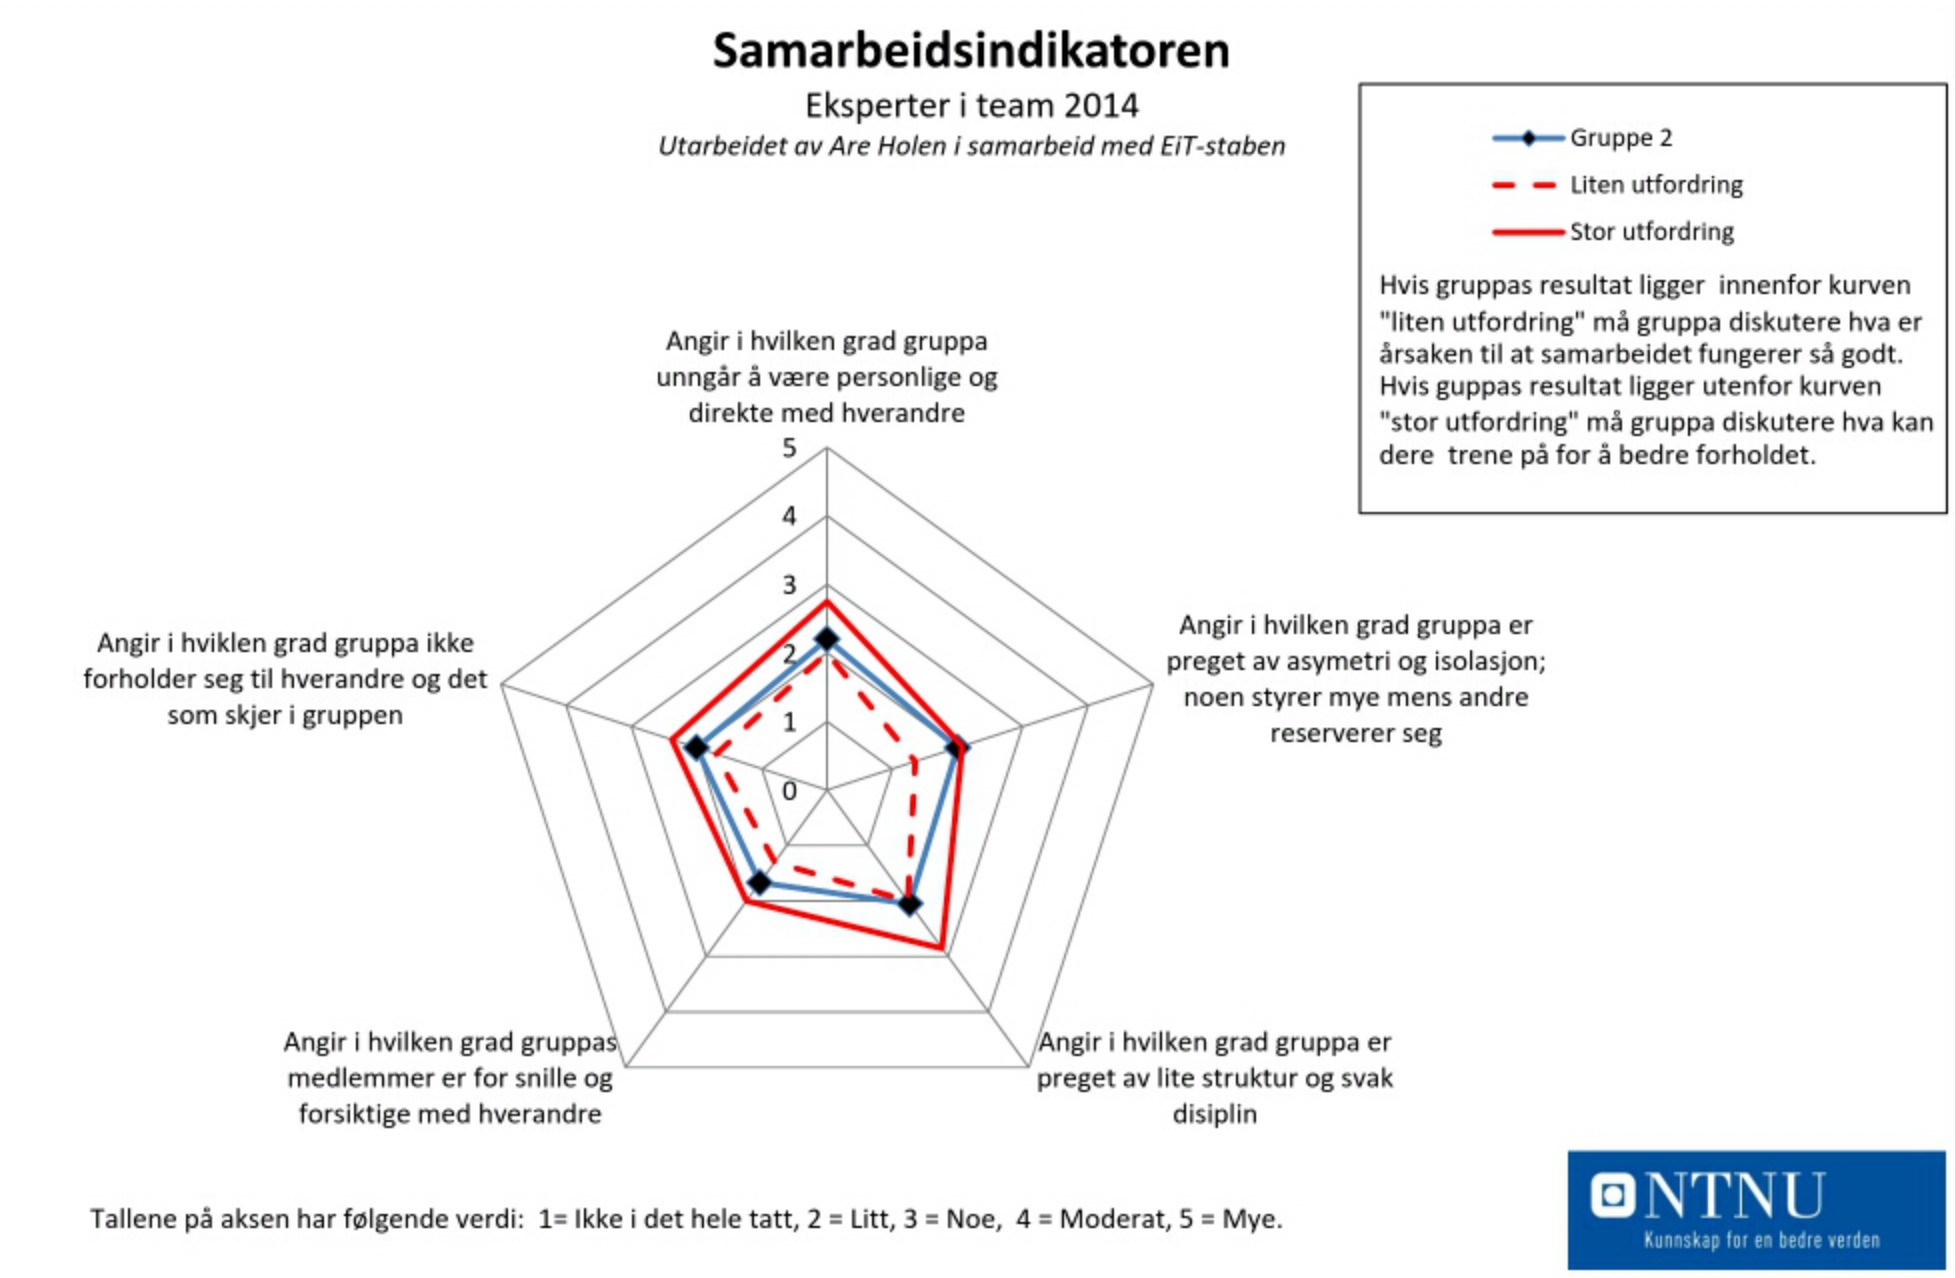
\includegraphics[width=0.7\textwidth]{images/samarbeidsindikator1.jpeg}	
    \caption{Samarbeidsindikatorer 2. landsbydag}
    \label{fig:sam1}
\end{figure}

\noindent \textbf{Hvilken grad gruppen unngår å være personlig:} 2.2.
\newline
\noindent Gruppen ligger mellom liten utfordring (1) og stor utfordring (nesten 3).
\vspace{\secspace}

\noindent \textbf{hvilken grad gruppen er preget av asymetri ogisolasjon:} 2.
\newline
\noindent Blablabla
\vspace{\secspace}

\noindent \textbf{Hvilken grad gruppen er preget av lite struktur:} 1.
\newline
\noindent Blablabla
\vspace{\secspace}

\noindent \textbf{Hvilken grad gruppen er for snille med hverandre:} 1.8.
\newline
\noindent Blablabla
\vspace{\secspace}

\noindent \textbf{Hvilken grad gruppen ikke forholder seg til hverandre:} 1.
\newline
\noindent Blablabla

\subsection{10. landsbydag}
\begin{figure}[H]
    \centering
    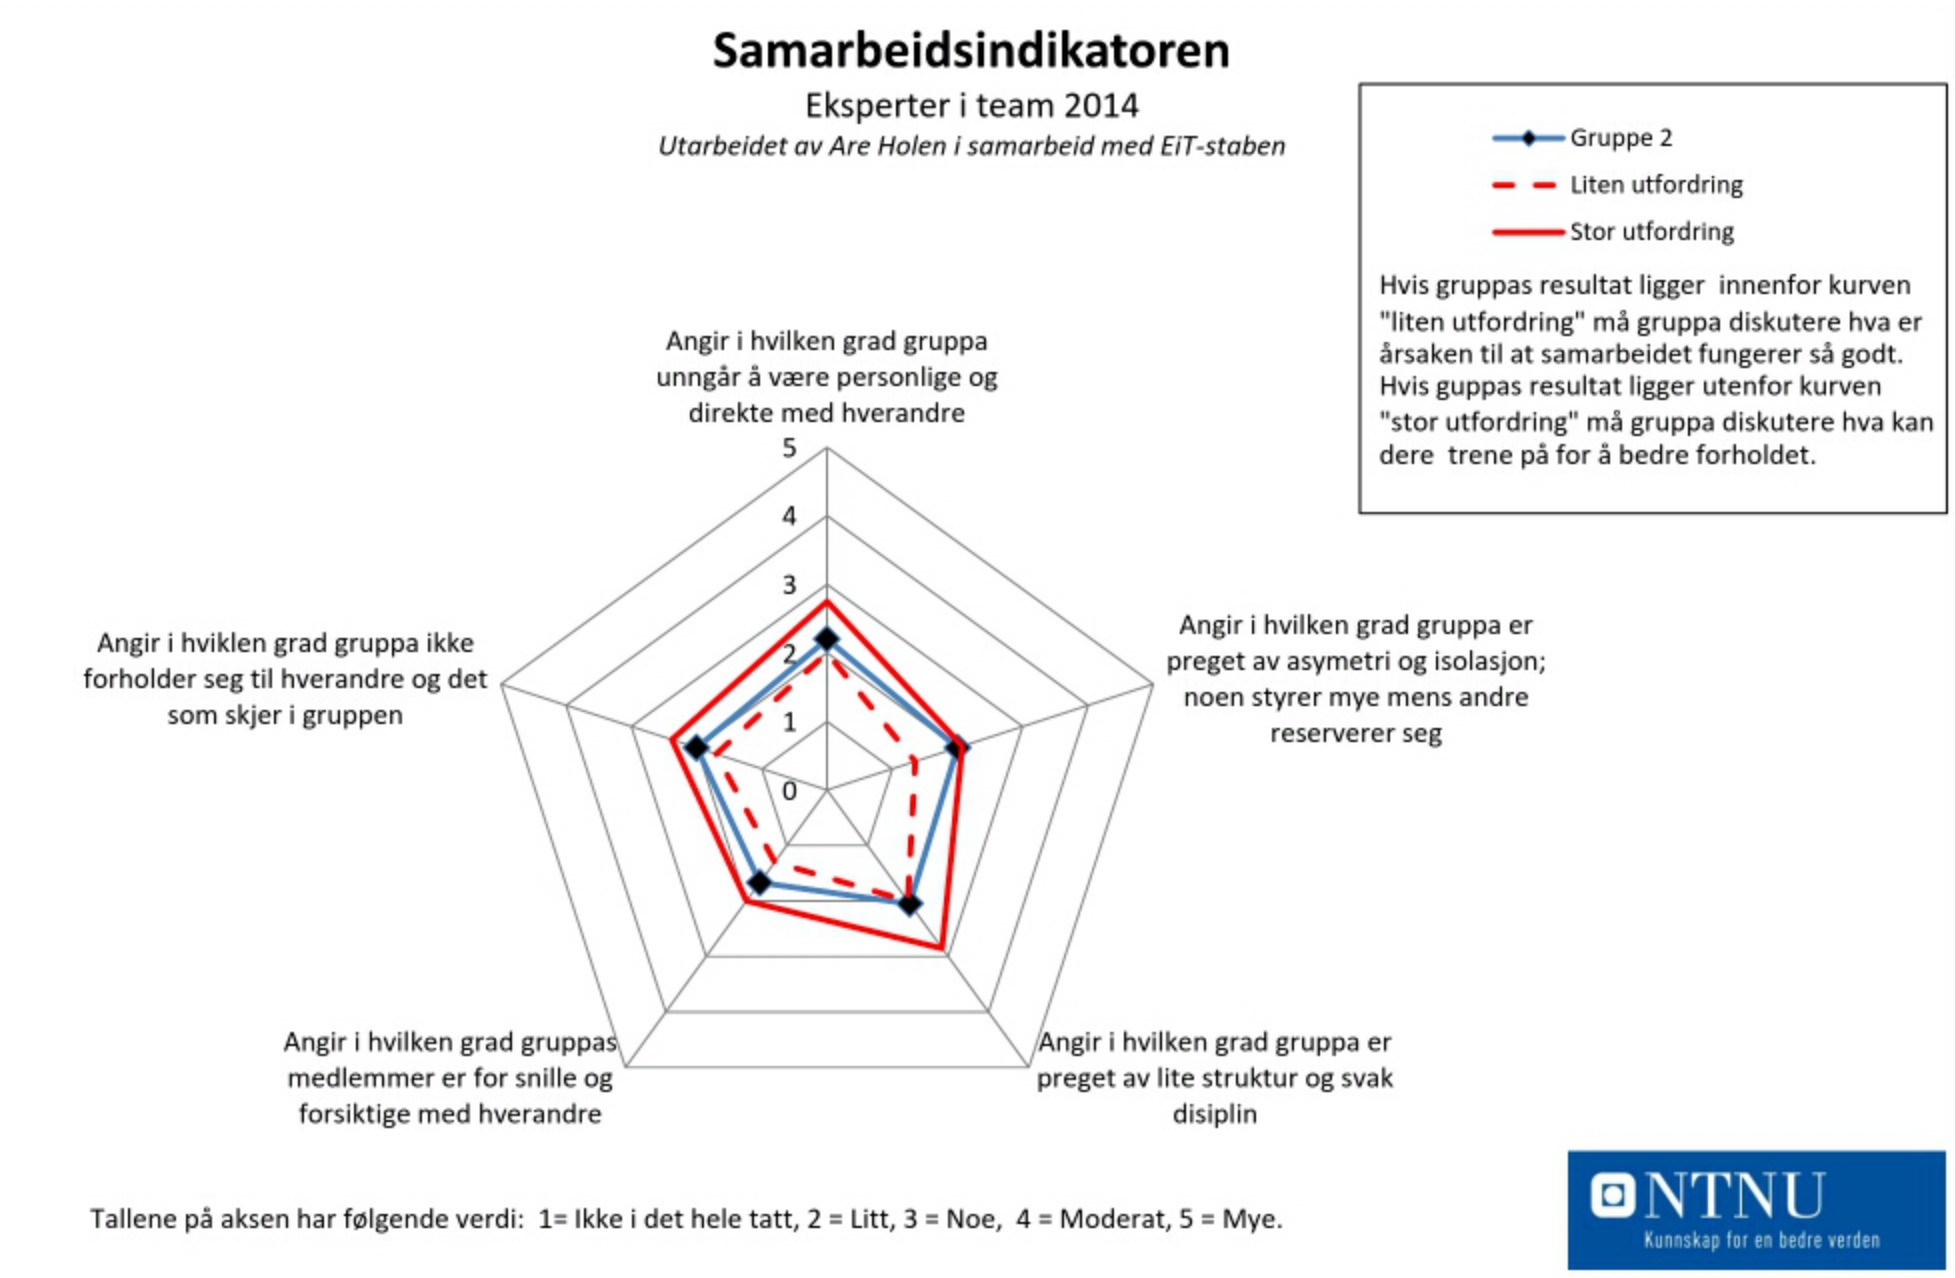
\includegraphics[width=0.7\textwidth]{images/samarbeidsindikator1.jpeg}	
    \caption{Samarbeidsindikatorer 10. landsbydag}
    \label{fig:sam2}
\end{figure}
